% This work is the property of Aleksandr Salo,
% Student of Baylor University, Computer Science Department. 
% Copying or using without notifying me is not allowed. 
% Contact email is alexsalovrn@gmail.com

\documentclass{article}

\usepackage{fullpage}
\usepackage{url}
\usepackage{hyperref}
\usepackage{amssymb}
\usepackage{amsmath}
\usepackage{graphicx}
\usepackage{epstopdf}
\usepackage{epsfig}
\usepackage{caption}
\usepackage{subcaption}
\usepackage[]{mcode}


\newcommand*{\Perm}[2]{{}^{#1}\!P_{#2}}%
\newcommand*{\Comb}[2]{{}^{#1}C_{#2}}%
\newcommand{\mytilde}{\raise.17ex\hbox{$\scriptstyle\mathtt{\sim}$}}
\newcommand{\patheta}{\frac{\partial}{\partial \theta_j} }
\newcommand{\pathe}{\frac{\partial}{\partial \theta} }
\newcommand{\pathx}{\frac{\partial}{\partial X} }
\newcommand{\thetax}{\theta^T x}
\newcommand{\elll}{\ell(\theta)}
\newcommand{\nath}{\nabla_\theta}
\newcommand{\pelll}{\frac{\partial^2 \elll}{\partial \theta_j \partial \theta_k}}
\newcommand{\ith}{^{(i)}}
\newcommand{\gdafrac}{\frac{1}{(2\pi)^{n/2}|\Sigma|^{1/2}}\exp}

% Dr. Hamerly's customization
% tell Latex to use no paragraph indentation, but leave some space between
% paragraphs 
\setlength{\parindent}{0in}
\setlength{\parskip}{0.1in}

\title{Assignment 1}
\date{Due March 3, 2015}
\author{Aleksandr Salo}

\begin{document}
\maketitle

\section{Ridge regression (20 points)}
	\begin{enumerate}
		\item  Using vector notation, find a closed-form solution for the $\theta$ that minimizes the ridge regression cost	function.
		
		Rules of derivation and trace operator that we are going to use:
		\begin{enumerate}
			\item $\pathx (Tr(X^T B X)) = BX + B^TX$. Note: if $B = I$ then  $BX + B^TX = 2X$
			\item $tr(X^T) = tr(X)$
			\item $tr(ABC) = tr(CAB) = tr(BCA)$
			\item $\nabla_A tr(AB) = B^T$
		\end{enumerate}
		
		Minimizing the following cost function:
		$$J(\theta) = \frac{1}{2} (X\theta - y)^T (X\theta - y) + \frac{\lambda}{2}\theta^T \theta$$
		
		We first take the gradient With respect to $\theta$:
		\begin{align*}
		\nath J(\theta) &= \frac{1}{2}\nabla_\theta (\theta^T X^T X\theta - \theta^TX^Ty - y^TX\theta + y^Ty)
		+ \nath (\frac{\lambda}{2}\theta^T \theta)\\
		&= \frac{1}{2}\nath (tr (\theta^T X^T X\theta) - 2tr(y^TX\theta)) + \frac{\lambda}{2}\nath(tr(\theta^T \theta))\\
		&= \frac{1}{2} (X^T X\theta + X^T X\theta - 2X^Ty) + \frac{\lambda}{2}(2\theta)\\
		&= X^T X \theta - X^Ty + \lambda\theta
		\end{align*}
		
		Then setting gradient to zero:
		\begin{align*}		
		X^T X \theta + \lambda\theta &= X^Ty \\
		(X^T X  + \lambda I) \theta &= X^Ty\\
		(X^T X  + \lambda I)^{-1} (X^T X  + \lambda I) \theta &= (X^T X  + \lambda I)^{-1} X^Ty		
		\end{align*}
		
		We find $\theta$ that solves the equation:
		$$ \theta = (X^T X  + \lambda I)^{-1} X^Ty $$
		
		\pagebreak
		\item Implement ridge regression using the functions hwk ridge.m and hwk zscore.m on the prostate data
		provided. Show the effect of the parameter $\lambda$ on three things: 
		\begin{figure}[h]
			\centering
			\begin{subfigure}{.8\textwidth}
				\centering
				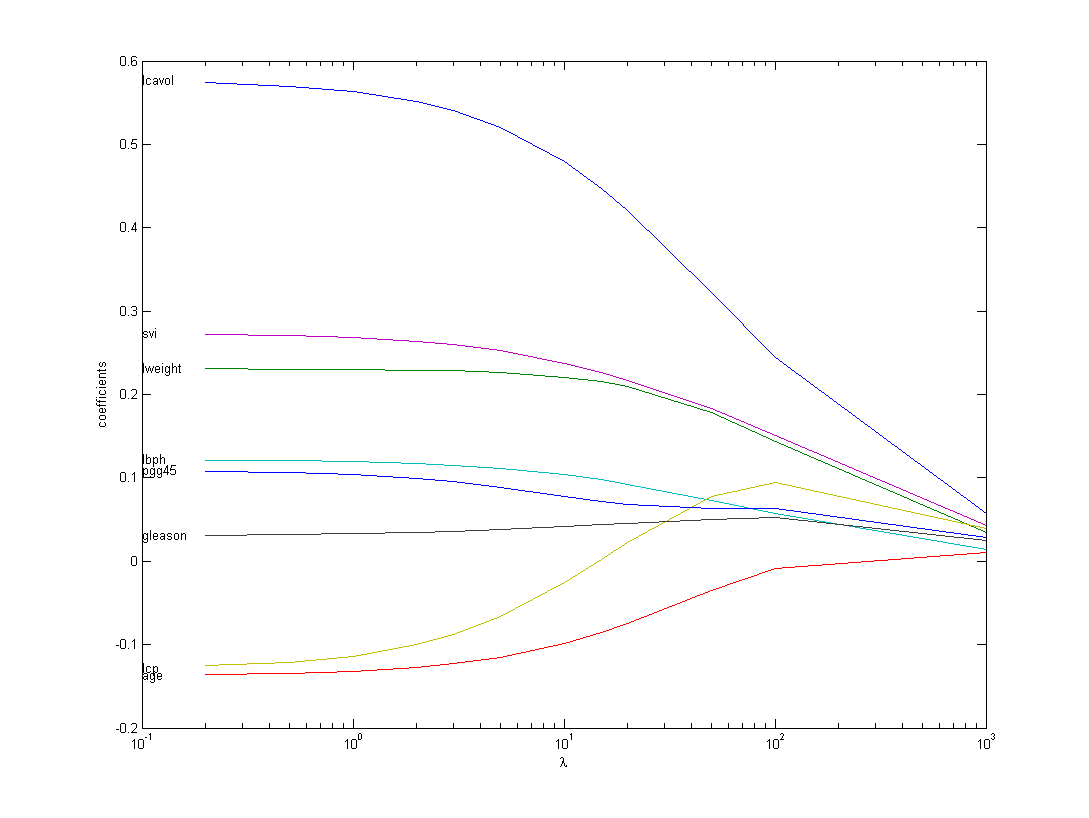
\includegraphics[width=.7\linewidth]{ridge_coeff.png}\
				\caption{Values of the individual components of $\theta$, $\lambda$ is log scaled}	
			\end{subfigure}
			\begin{subfigure}{.48\textwidth}
				\centering
				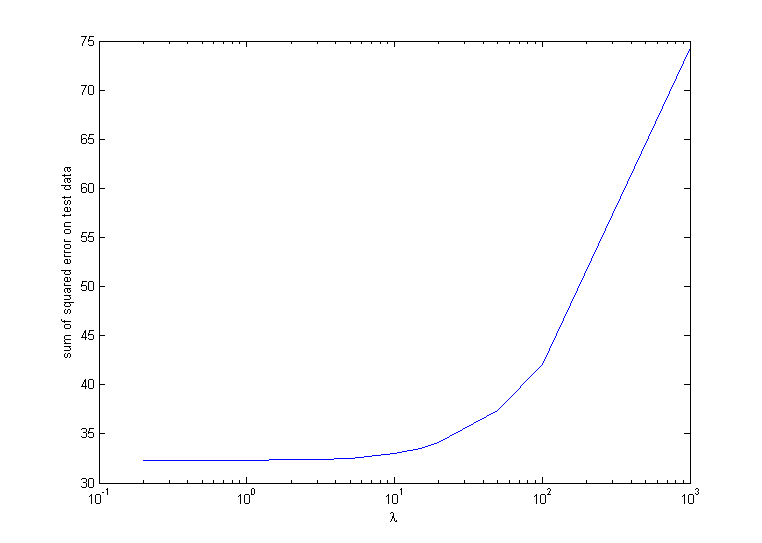
\includegraphics[width=.9\linewidth]{ridge_SLE.png}\
				\caption{Non-regularized cost function}	
			\end{subfigure}
			\begin{subfigure}{.48\textwidth}
				\centering
				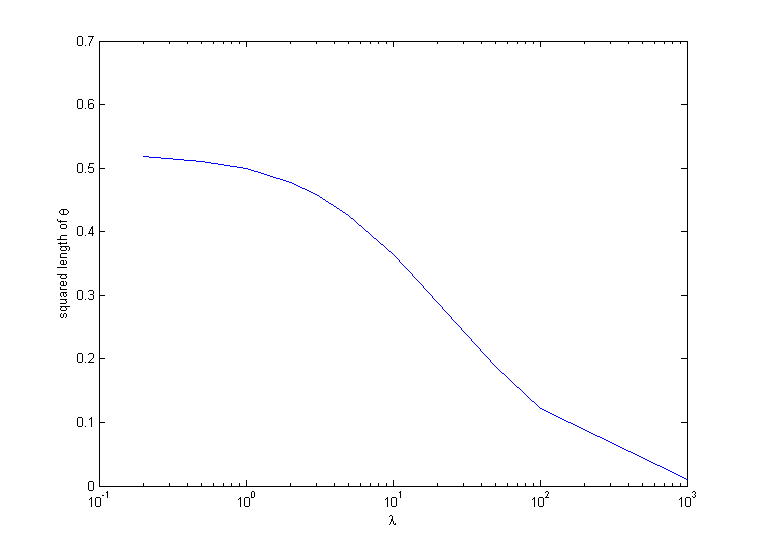
\includegraphics[width=.9\linewidth]{ridge_thetaSquared.png}\
				\caption{Value of $\theta^T \theta$}	
			\end{subfigure}
		\end{figure}	
		\begin{enumerate}		
		\item the values of the individual components of $\theta$:\\
			$\lambda$ restricts the growth rate of $\theta$ components. The larger the value of $\lambda$, the greater the amount of shrinkage (that is to say that the coefficients become more robust to collinearity). Ultimately, with $\lambda=1000$ for provided dataset, all coefficients converge to a single value of zero. 
		
		\item the non-regularized cost function on held-out test data:\\
			Naturally, with bigger $\lambda$ and less diverse and less accurate $\theta$ cost function grows.\\
			However, when looking at te detailed behavior, it's clear that for provided dataset cost function really start to grow only since $\lambda=0.5$. Thus not significantly decreasing the accuracy of prediction by penalizing to high $\theta$ values.
		\item the value of $\theta^T \theta$:\\
			Obviously, at the same time the squared length of theta decreases.
		\end{enumerate}
		
		Thus ridge regression technique allows to penalize high theta coefficients (that appeared due to potential collinearity in the data) while with moderate values of parameter $\lambda$ it would not significantly decrease predictive power (in other words would not increase cost function). By doing that we avoid blown-up theta values that potentially lead to calculus errors. 
	\end{enumerate}

\pagebreak	
\section{Gaussian Discriminant Analysis (30 points)}
	\begin{enumerate}		
		\item Find optimal $\mu, \phi$ by maximizing log-likelihood of the following input data model:
		$$p(x|y=0; \mu^0, \Sigma) = \gdafrac(-\frac{1}{2}(x-\mu^0)^T\Sigma^{-1} (x-\mu^0)) $$
		$$p(x|y=1; \mu^1, \Sigma) = \gdafrac(-\frac{1}{2}(x-\mu^1)^T\Sigma^{-1} (x-\mu^1)) $$
		$$p(y; \phi) = \phi^y(1-\phi)^{1-y}$$
		
		Which gives the following joint likelihood:
		\begin{align*}
		L(\phi, \mu^0, \mu^1, \Sigma) &=  \prod_{i=1}^{m} p (x\ith, y\ith; \phi, \mu^0, \mu^1, \Sigma) \\
		&=  \prod_{i=1}^{m} p (x\ith | y\ith; \mu^0, \mu^1, \Sigma) p(y\ith; \phi)
		\end{align*}
		
		Taking the log-likelihood allows us to break product into sum:\\
		$$\ell(\phi, \mu^0, \mu^1, \Sigma) = \sum_{i=1}^{m} p (x\ith | y\ith; \mu^0, \mu^1, \Sigma) p(y\ith; \phi)$$
		
		Now we take partial derivatives and set it to zero to find the MLEs.\\
		\textbf{With respect to $\phi$}:
		\begin{align*}
		0 &=\frac{\partial}{\partial \phi} \sum_{i=1}^{m} (y\ith log \phi + (1-y\ith)log(1-\phi))\\
		&= \frac{1}{\phi} \sum_{i=1}^{m}y\ith - \frac{1}{1 - \phi} \sum_{i=1}^{m}(1 - y\ith)\\
		\frac{1}{\phi} \sum_{i=1}^{m}y\ith &= \frac{1}{1 - \phi} \sum_{i=1}^{m}(1 - y\ith)\\
		\phi \sum_{i=1}^{m}1 - \phi \sum_{i=1}^{m}y\ith &= \sum_{i=1}^{m}y\ith - \phi \sum_{i=1}^{m} y\ith\\
		\phi &= \frac{\sum_{i=1}^{m}y\ith}{m} \\
		\phi_{optimal} &= \frac{1}{m} \sum_{i=1}^{m} 1 \{y\ith = 1\}
		\end{align*}	
		
		\pagebreak
		\textbf{With respect to $\mu^0$}:\\
		\begin{align*}
		0 &=\frac{\partial}{\partial \mu^0} \sum_{i=1}^{m} -\frac{1}{2}(x\ith-\mu^0)^T\Sigma^{-1} (x\ith-\mu^0)\\
		&= \sum_{i=1}^{m} -\frac{1}{2} (x\ith-\mu^0)^T (\Sigma^{-1} + (\Sigma^{-1})^T)(-1)\\
		&= \sum_{i=1}^{m} \Sigma^{-1} (x\ith-\mu^0)^T 
		\end{align*}
		Note, that:
		\begin{enumerate}		
			\item $\frac{\partial}{\partial x} x^T Ax = x^T(A+A^T)$
			\item Covariance matrix $\Sigma$ is symmetric around main diagonal, hence $\Sigma = \Sigma^T$
		\end{enumerate}
		
		\item Prove that for two-class Gaussian Discriminant Analysis, with common covariance $\Sigma$, the posterior probability $p(y=1|x;\phi, \mu^0, \mu^1, \Sigma)$ is a logistic sigmoid function $g(z) = 1/(1+exp(-z))$.\\
		By Bayes' Rule:
		$$	p(y=1|x) = \frac{p(x|y=1)p(y=1)}{p(x|y=1)p(y=1) + p(x|y=0)p(y=0)}$$
		Let:
		\begin{enumerate}
			\item $p(x|y=1)p(y=1) = A$
			\item $-\frac{1}{2}(x-\mu^0)^T\Sigma^{-1} (x-\mu^0) = -z$
			\item $\frac{1}{(2\pi)^{n/2}|\Sigma|^{1/2}} = c$
		\end{enumerate} 
		Then:
		$$	 = \frac{A}{A + c \cdot e^{-z}}$$
		Now divide the entire fraction by $A$:
		$$	 = \frac{1}{\frac{A + c \cdot e^{-z}}{A}}$$
		Divide denominator by parts:
		$$= \frac{1}{1 + c \cdot e^{-z}}$$
		Which is exactly sigmoid function.
		
		\item Implementation of Gaussian discriminant analysis gives the following results:\\
		\textbf{Base Rate Accuracy:} 0.0909 which means, that if we are just to guess the class label we would have ~9 \% chance to guess correctly. \\	
		\textbf{Training Data Accuracy:}  0.6818 that is to say, that when we try to predict on data that we used for learning, we get 68\% chance of predicting correctly. That is on 59\% better than the base case, which is significant learning result \\	
		\textbf{Test Data Accuracy:}  0.4437 that is to say, that when we try to predict on the brand new data we get 44.5\% chance of predicting correctly. That is on 36.5\% better than the base case, yet it significantly worse than predicting on train data\\
		\textbf{Per class accuracy:} Not surprisingly, precision differs for different classes:\\
		\begin{table}[h!]	
			\begin{center}	
			\begin{tabular}{l l l}
				Class & Train Data & Test Data \\ \hline
				1 & 0.6458		 &    0.6667
				\\  2 &   0.5833 		 &    0.3810
				\\ 3 &   0.8750		 &    0.3810
				\\ 4 &   0.7500		 &    0.7857
				\\  5 &  0.6875		 &    0.1667
				\\   6 & 0.4792		 &    0.4524
				\\    7 & 0.6875		 &    0.2619
				\\    8 & 0.7083		 &    0.5476
				\\    9 & 0.6042		 &    0.3571
				\\    10 & 0.6875		 &    0.3095
				\\    11 & 0.7917		 &    0.5714
				
			\end{tabular}
			\end{center}
		\end{table}	
	\end{enumerate}

\pagebreak
\section{Optimal margin classifier (10 points)}
The optimal margin classifier is the one which maximizes the geometric margin separating examples from
the two classes. This is defined as:
$$ \min_{w,b} ||w||^2  $$
$$ \forall i: y\ith (w^Tx\ith +b) \ge 1  $$
\begin{enumerate}
	\item Prove that $w$ is orthogonal to the decision hyperplane (the hyperplane is the set of points ${x|w^Tx+b=0}$). Recall that two vectors $u$ and $v$ are orthogonal iff $u^Tv= 0$.
	\begin{enumerate}
		\item Vector is orthogonal to a plane if it is orthogonal to a vector that belongs to a plane
		\item Rewrite the equation of hyperplane: $w^Tx = -b$
		\item When $b=0$, the hyperplane H is simply set of points that are orthogonal to $w$; when $b\neq 0$, the hyperplane is a translation, along the direction $w$, of that set. 
		\item For the equation above, $w^T$ and $b$ are given, and then different x's, that solve the equation, for the hyperplane H: if $x_0 \in H$ then for any other $x \in H$:
		\begin{align*}
		-b = w^Tx_0 &= w^Tx\\
		-b - w^Tx_0 &= w^Tx - w^Tx_0\\
		-b - (-b) &= w^T(x - x_0)\\
		0 &= w^T(x - x_0)
		\end{align*}
		Thus a the hyperplane can be expressed as the set of vectors $x$ s.t. $x-x_0$ is orthogonal to $w$
		\item Taken into account this description, \textit{any} vector from hyperplane is orthogonal to $w$, hence $w$ is orthogonal to hyperplane itself.
	\end{enumerate}
	
	\item The equation $w^Tx+b=0$ forms a single hyperplane in the feature space of the variables x, with normal
	vector $w$. However, when thinking about minimizing the objective $w^Tw$ subject to the $m$ constraints
	$y\ith (w^Tx\ith +b) \ge 1$, we said that each constraint forms a (different) hyperplane that separates the
	feasible and non-feasible space of solutions. Explain why each constraint's shape is a hyperplane, and
	why each of the $m$ constraints makes a different hyperplane (when we have a single hyperplane for the
	decision boundary).
	
	\begin{enumerate}
		\item Since a hyperplane is a the set of points x s.t. $w^Tx+b=0$  if we have an m different equations $w^Tx\ith +b=0$ we have m different hyperplanes (for m different x's). 
		\item For the decision boundary we have a single hyperplane because we form it in the space of X thus making one optimal w.\\
		On contrary, in space of w, each example of X forms its own hyperplane. Different x's hyperplanes intersect and form the space in which w could take its value to be optimal.\\
		So answer is really is: because we have multiple x vectors and only one w vector. 
	\end{enumerate}
	
\end{enumerate}



\pagebreak
\section{Naive Bayes and SVMs for Text Classiffication (20 points)}	
\begin{enumerate}
	\item Naive Bayes Multinomial classifier performance using each of the different training files
	(but each time using the same test file) give the following error rate.
	\item The same for SVM classifier + comparison of classifiers:
	\begin{figure}[h!]
		\centering		
		\begin{subfigure}{.45\textwidth}
			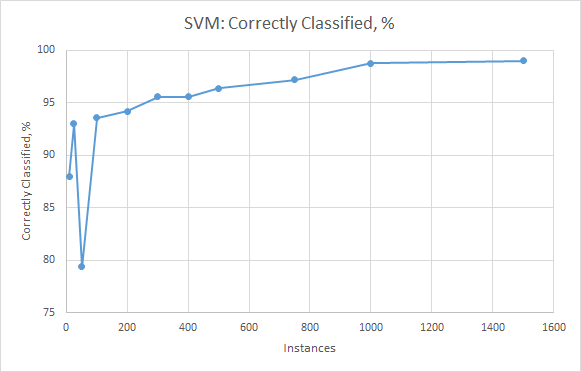
\includegraphics[width=1\linewidth]{SVM_spam.png}\
			\caption{Naive Bayes Spam Filter}	
		\end{subfigure}
		\begin{subfigure}{.45\textwidth}
			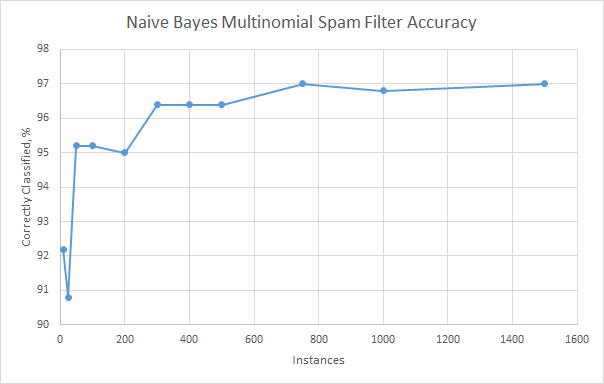
\includegraphics[width=1\linewidth]{NBM_spam.png}\
			\caption{SVM Spam Filter}	
		\end{subfigure}
		\begin{subfigure}{.7\textwidth}
			\centering
			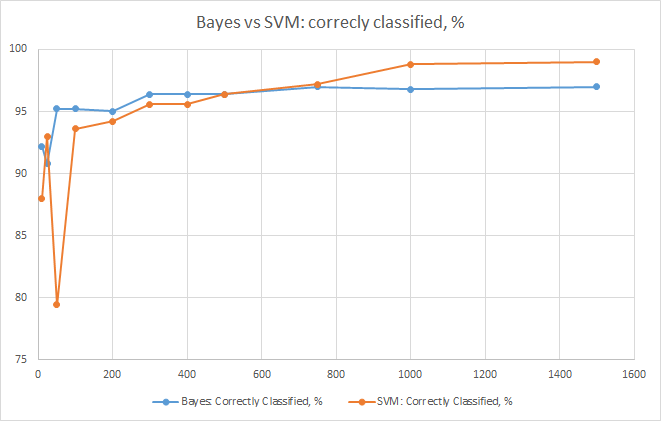
\includegraphics[width=1.1\linewidth]{NBM_SVM_spam.png}\
			\caption{Naive Bayes vs SVM accuracy}	
		\end{subfigure}		
	\end{figure}	

	For Naive Bayes, accuracy is good from the beginning (with only 10 training examples), gets even better after 300 examples, and then don't improve significantly. \\
	
	For SVM, although accuracy is good from the beginning, it seems like it less robust with small amount of examples. However, after 500 training examples, SVM significantly outperforms Bayes classified in prediction accuracy. 
	
	\item Consider the issue of estimating the multinomial probability of seeing a word w by using a training set
	with m examples.\\
	If the training contains b(w) occurrences of w, then the MLE is:
	$$P(w)= \frac{b(w)}{m} $$
	If b(w)=0 then P(w) = 0, thus adding Laplace-smoothing:
	$$P(w)_{laplace}=\frac{b(w) + 1}{m + d}$$
	Thus, Laplace smoothing raises the probability of words that would have zero probability.\\
	Intuitively, for other words in the dictionary it could significantly bring probability down. For example, we have a email which contains: "The quick brown fox", and our dictionary consists of 30000 words. That gives:
	$$P("fox")= \frac{1}{4}; P("propagotary")= \frac{0}{4} = 0 $$
	$$P("fox")_{laplace}=\frac{2}{30004}; P("propagotary")_{laplace}=\frac{1}{30000}$$
	Prior the Laplace Smoothing, word "fox" was infinitly more likely to occur than "propagotary" according to our model. After smoothing, it became twice more likely to occur, which makes sense.
	
\end{enumerate}
	
	
     
\end{document}